
%================================
\subsection{Resultados del algoritmo paralelizado con hilos}
\label{sec:Resultados_hilos}

Para esta implementación se utilizó la biblioteca de hilos POSIX (pthreads) para crear múltiples hilos que ejecutan el algoritmo de Jacobi en paralelo. Cada hilo se encarga de procesar una parte del arreglo, lo que permite aprovechar la capacidad de procesamiento de múltiples núcleos del CPU. Se realizaron pruebas con diferentes números de hilos (2, 4, 6, 8 y 12) para evaluar el impacto en el rendimiento. Estos fueron los resultados obtenidos:

\begin{table}
   \centering
   
\includegraphics{images/tables/threads_time.png}
   \caption{Resultados del algoritmo paralelizado con hilos}
   \label{tab:threads}
\end{table}

\begin{table}[H]
   \centering
   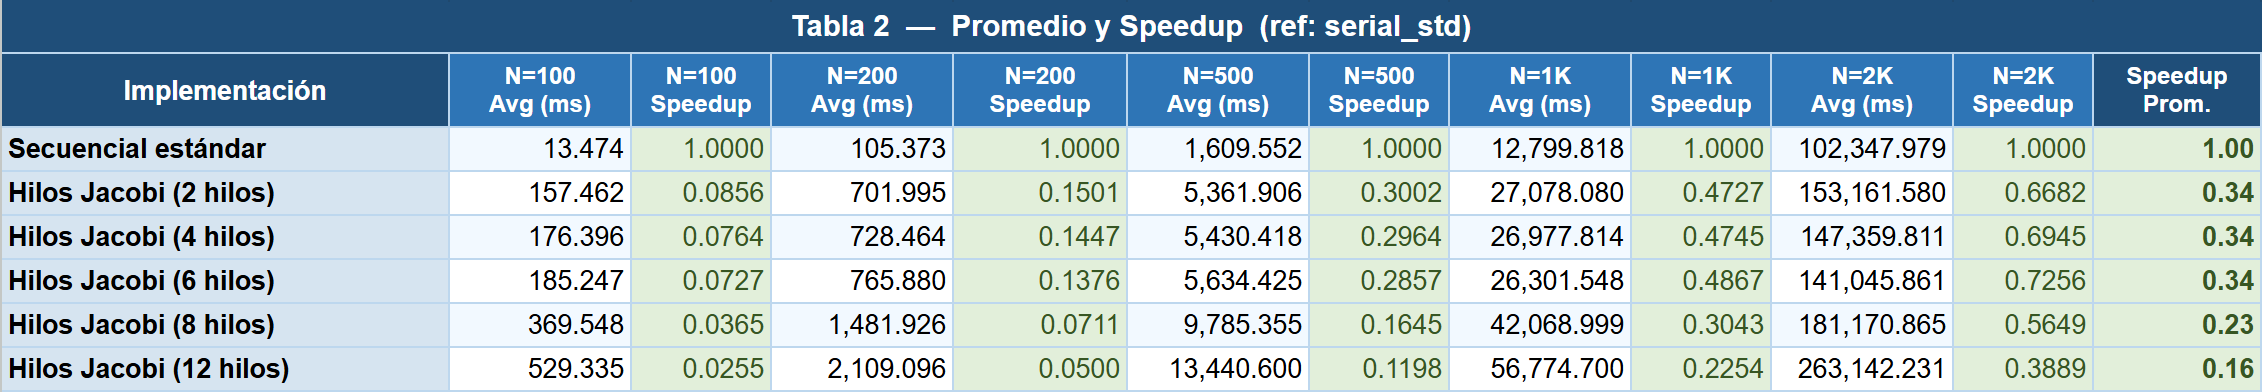
\includegraphics[width=1\textwidth]{images/tables/threads_speedup.png}
   \caption{Speedup del algoritmo paralelizado con hilos}
   \label{tab:threads_speedup}
\end{table}

\begin{figure}[H]
   \centering
   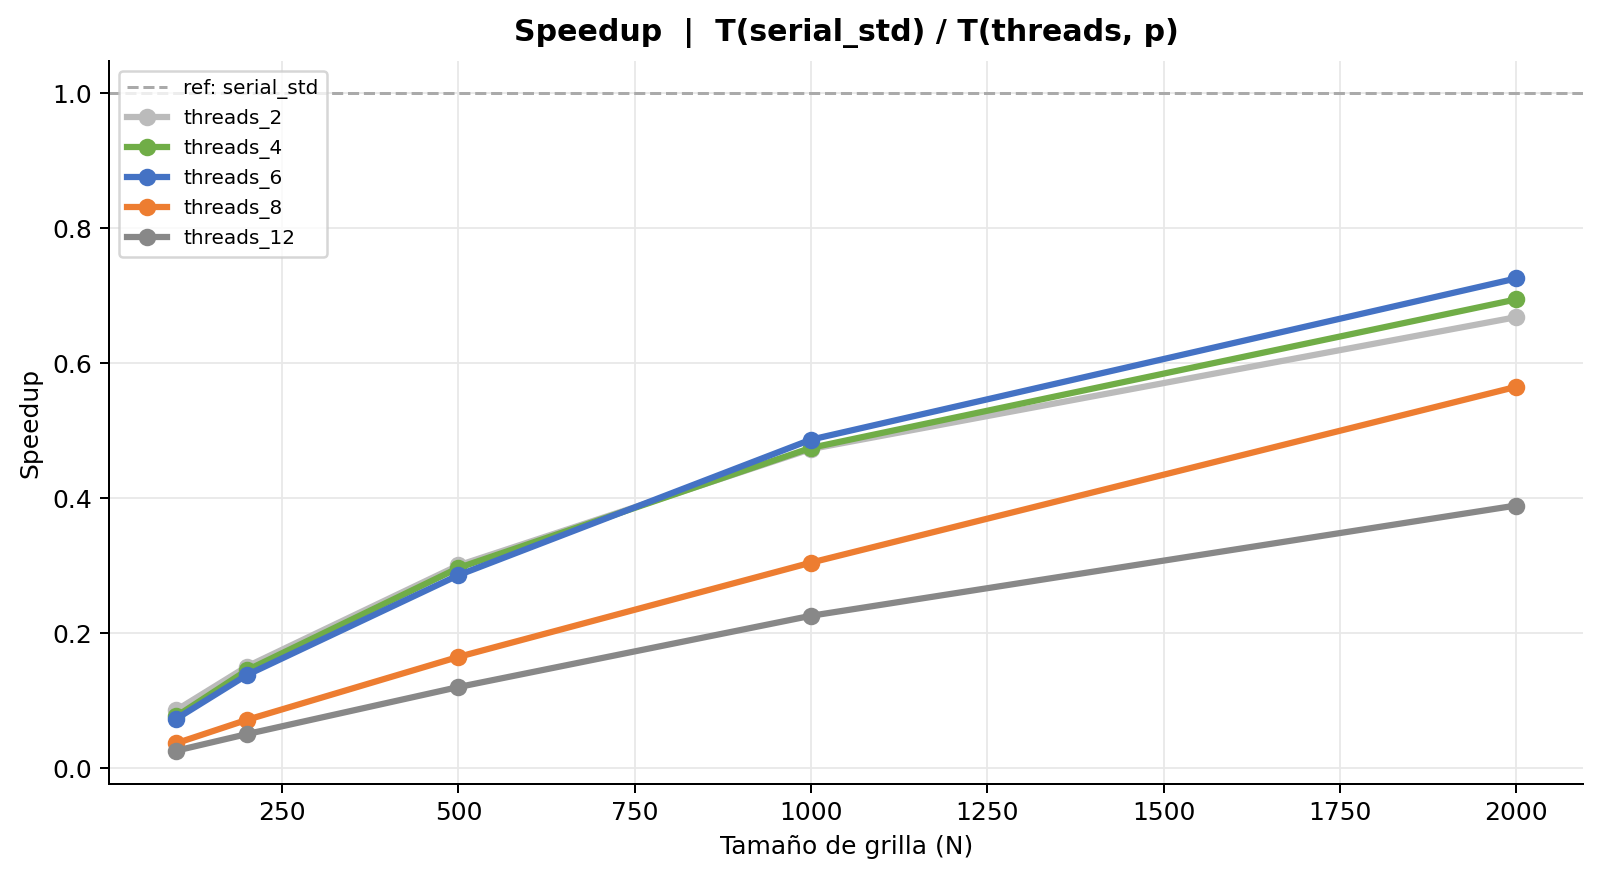
\includegraphics[width=1\textwidth]{images/charts/threads_sp.png}
   \caption{Comparación del speedup entre el algoritmo secuencial y el algoritmo paralelizado con hilos}
   \label{fig:chart_threads_speedup}
\end{figure}